
%======================问题介绍====================================
\section{Introduction}
In bidirectional traffic, right- and left-hand traffic requires 
vehicles keep either to the right or the left side of the road, 
respectively.\cite{Draper_Geoff_1993} The first right-hand 
traffic law in United State dates back to 1792, applied to the 
Philadelphia and Lancaster Turnpike.\cite{Weingroff_Richard_2014}\\

The right-hand traffic rule derives regulations on multi-lane 
freeways, which often requires drivers to drive in the 
right-most lane unless they are passing another vehicle, in 
which case they move one lane to the left, pass, and return 
to their former travel lane. The overtaking lane provides 
redundant convenience and safety for vehicles to pass others, 
but lowers freeway's traffic flow capability.\\

Different models may exist that provide a better tradeoff 
among traffic flow, safety and convenience. This paper 
considers these three criteria, introduces a different 
freeway traffic model and analyses performances of the two 
models.


\subsection{Other Assumptions}

\begin{itemize}
\item
\item
\item
\item
\end{itemize}

 Under the above and basic assumptions, we can set out
to construct our model (show our approach in detail).
%=============================问题分析==========================================
\section{Analysis of the Problem }
We are going to evaluate the right-most rule' performance from two aspects: the safety and the traffic flow.
\subsection{safety}
\emph{Assumptions}
\begin{itemize}
\item The value of acceleration subjects to normal distribution, $\mu = \frac{max(a)}{2}$,
$\sigma = \frac{1}{4}\mu$, for $p(0 < a_2 < \frac{1}{4} \mu)$ and $p(\frac{7}{4} \mu < a_2 < 2\mu)$ is very small.
\end{itemize}

%==================================模型建立==============================================
\paragraph{Safe Distance Model}

On the highway, if the car in front suddenly slows down, it is likely that a car crash happens.
We build this model to calculate the safe distance between two adjacent cars. That is ,
if the adjacent $d \leq l$ and the car in front suddenly slows down,the accident will not happen.\\ \\
\begin{table}
\centering
\begin{tabular}{ll}
\hline
Parameter & Meaning\\
\hline
$a_1$ & the acceleration of the  car in behind \\
$v_1$ & the velocity of the  car in front \\
$a_2$ & the acceleration of the car in front \\
$v_1$ & the velocity of the  car in front \\
$t_r$ & the driver's reaction time \\
$t$ & the total time whole process \\
$l$ & the safe distance \\
$d$ & a constant which is the real distance between the car in front and the car in behind.\\
\hline
\end{tabular}
\caption{Model parameter}
\end{table}

\begin{figure}[h]
\small
\centering
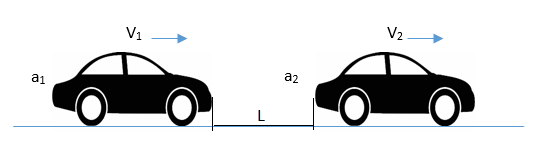
\includegraphics{situation.png}
\caption{} %\label{fig::collision}
\end{figure}

There are two possible situations that the accident will happen:
\begin{itemize}
\item The accident happens after the car in front stopped.
That is, when
\begin{displaymath}
\frac{v_2}{a_2}  \geq  \frac{v_1}{a_1} + t_r
\end{displaymath}
We have:
\begin{eqnarray}
\frac{v_1^2 - v_0 ^ 2}{2a_1} + v_1 t_r - l & = & \frac{v_2 ^ 2 - v_0 ^ 2}{2a_2}\\
\frac{v_2 - v_0}{a_2} & = & t\\
\frac{v_1 - v_0}{a_1} & = & t - t_r
\end{eqnarray}
\item The collision happens before the car in front stopped. That is, when
\begin{displaymath}
\frac{v_2}{a_2}  >  \frac{v_1}{a_1} + t_r
\end{displaymath}
We have:
\begin{eqnarray}
v_1 t_r + \frac{v_1 ^ 2}{2a_1} - l& = &\frac{v_2^2}{2a_2}
\end{eqnarray}
\end{itemize}

Solve this equation array, we have
\begin{displaymath}
l(a_1, a_2, v_1, v_2) = 
\left \{
\begin{array}{cl}
\dfrac{(a_1a_2t_r^2 + 2a_1t_rv_2 + v_1^2 - 2v_1v_2 + v_2^2)}{2(a_1-a_2)} & \dfrac{v_2}{a_2}  \geq \dfrac{v_1}{a_1} + t_r \\
v_2 t_r + \dfrac{v_1 ^ 2}{2a_1} -\dfrac{v_2^2}{2a_2} & \dfrac{v_2}{a_2}  < \dfrac{v_1}{a_1} + t_r
\end{array}
\right .
\end{displaymath}
\\

To calculate $l_{max}$, firstly, we are going to find the extrema,

\begin{displaymath}
\left \{
\begin{array}{cl}
\dfrac{\partial l}{\partial{a_1}} = 0 \\
\dfrac{\partial l}{\partial{a_2}} = 0 \\
\dfrac{\partial l}{\partial{v_1}} = 0 \\
\dfrac{\partial l}{\partial{v_2}} = 0 \\
\end{array}
\right .
\end{displaymath}

This equation array has no solution, which indicates that we can get the $l_{max}$ at the boundary of domain.

$l$ reaches the maximum when $a_1$ equals to $a_{min}$, { }$v_1$ equals to $v_{1max}$, $v_2$ equals to $v_{2min}$. (If the front car drives with the lowest speed, the rear car drives with the highest speed, and at the same time, rear car's acceleration is the minimum, when emergency happens, the braking distance is the longest.)

Thus, we have:
\begin{displaymath}
l_{max}(a_2) = 
\left \{
\begin{array}{cl}
\dfrac{(a_{min}a_2t_r^2 + 2a_{min}t_rv_{min} + v_{max}^2 - 2v_{max}v_{min} + v_{min}^2)}{2(a_{min}-a_2)} & \dfrac{v_{min}}{a_2}  \geq \dfrac{v_1}{a_1} + t_r \\
v_{min} t_r + \dfrac{v_{max} ^ 2}{2a_{min}} -\dfrac{v_{min}^2}{2a_2} & \dfrac{v_2}{a_2}  < \dfrac{v_1}{a_1} + t_r
\end{array}
\right .
\end{displaymath}\\

\paragraph{$l${ } Distribution}
From the result above, we can get $a_2(l)$

%\usepackage{amsmath}
\[ a_2(l) = \begin{cases}
-\dfrac{v_{max}^2 - 2v_{max}v_{min} + 2a_{min}t_rv_{max} + v_{min}^2 - 2a_{min}t_rv_{min} - 2la_{min}}{a_{min}t_r^2 + 2l}, 
\\

\quad l \leq \dfrac{v_{max}^2 - v_{max}v_{min} + 2v_{max}a_{min}t_r - a_{min} v_{min}t_r}{2a_{min}}\\
\dfrac{a_{min}v_{min}^2}{v_{max}^2 + 2a_{min}t_rv_{max} - 2la_{min}}, \quad  l > \dfrac{v_{max}^2 - v_{max}v_{min} + 2v_{max}a_{min}t_r - a_{min} v_{min}t_r}{2a_{min}}
\end{cases}\]
\\
\paragraph{Safety Factor $\alpha$}
For every car, it has a unique safety factor $\alpha$, the closer the distance between two adjacent cars is, the smaller the $\alpha$ is, vice versa.\\
\begin{figure}[h]
\small
\centering
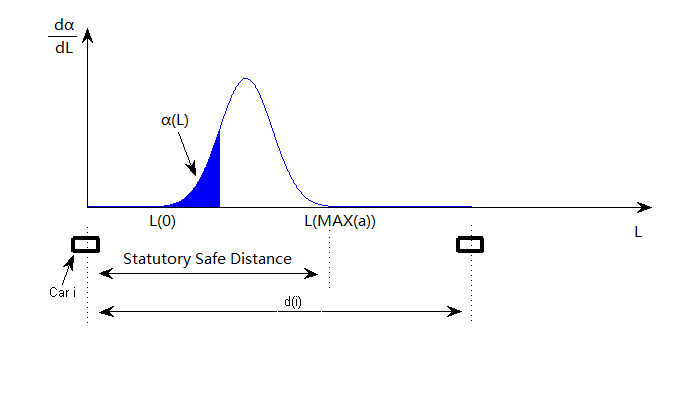
\includegraphics{draw_SafetyNormalDistribution_graph.png}
\caption{safety factor distribution} \label{fig::safety factor distribution}
\end{figure}
\begin{displaymath}
\alpha(l) = \int_{0}^{l} f(x) dx.
\end{displaymath}
%\textbf{Assumptions}\\
%\begin{itemize}
%\item d is the distance between two adjacent cars.
%\end{itemize}
We can see that , when $a_2$ = 0, that is, the front car has the lowest deceleration. Since $l(a)$ is a monotone increasing function, at this time,$l$ is minimal. In other word, it is of little possibility that the distance is less than the l, that is, $\alpha(l) \rightarrow 0$                     

\subsection{traffic flow}
Since the layout of the cars on the freeway is complicated, to simplify, we use a special model to discuss the relationship between the safety and traffic flow under the situation with and without the right-most rule.
\\
\paragraph{Assumption}
\begin{itemize}
\item Only one car are overtaking, the others are driving with a constant speed
\item Every overtaking, pass only one car
\end{itemize
\begin{itemize}
\item the rest flow on a single lane
\begin{equation}
J^* = J_{supply} - J_{need}
\end{equation}
\item 
\[ J^* = \begin{cases}
0,\\
\bar{l} - \bar{l}_{max}
\end{cases}\]

\item Without the right-most rule, there is no overtaking lane, vehicle can stay on either lane at any time.
\item On the freeway, except the overtaking car, others are subject to the uniform distribution.
\end{itemize}


\begin{displaymath}
\beta = A\beta_1 + B\beta_2
\end{displaymath}
(A, B are weight)

\begin{itemize}
\item 
\begin{displaymath}
\beta_1 = \frac{J_1 - J_2}{J_2}
\end{displaymath}
\end{itemize}

\begin{table}
\centering
\begin{tabular}{ll}
\hline
Parameter & Meaning\\
\hline
$J$ & traffic flow\\
$J_1$ & the supply traffic flow \\
$J_2$ & the demand traffic flow \\
$s$ & the lenth of a car \\
$l$ & the safe distance \\
$\bar{v}$ & the average velocity\\
\hline
\end{tabular}
\caption{Model parameter}
\end{table}
Supply
Demand
\section{Calculating and Simplifying the Model  } ``A is equivalent
to B'' Although Mr. Gore has expressed concerns to some associates
about the damage a brokered convention could cause, several
associates said he was hopeful that one candidate would soon break
through, sparing the party such an outcome. He told a close friend
recently that his decision not to endorse ``feels like the right
thing'' and that he remained optimistic the race ``is going to tip
at some point,'' the friend said.



%===============================模型结果============================================
\section{The Model Results}
Although Mr. Gore has expressed concerns to some associates about
the damage a brokered convention could cause, several associates
said he was hopeful that one candidate would soon break through,
sparing the party such an outcome. He told a close friend recently
that his decision not to endorse ``feels like the right thing''
and that he remained optimistic the race ``is going to tip at some
point,'' the friend said.


%========================模型的实效分析(适应性说明)=============================

\section{Validating the Model}%确认模型,使之合理。
Although Mr. Gore has expressed concerns to some associates about
the damage a brokered convention could cause, several associates
said he was hopeful that one candidate would soon break through,
sparing the party such an outcome. He told a close friend recently
that his decision not to endorse ``feels like the right thing''
and that he remained optimistic the race ``is going to tip at some
point,'' the friend said. Although Mr. Gore has expressed concerns
to some associates about the damage a brokered convention could
cause, several associates said he was hopeful that one candidate
would soon break through, sparing the party such an outcome. He
told a close friend recently that his decision not to endorse
``feels like the right thing'' and that he remained optimistic the
race ``is going to tip at some point,'' the friend said.


Although Mr. Gore has expressed concerns to some associates about
the damage a brokered convention could cause, several associates
said he was hopeful that one candidate would soon break through,
sparing the party such an outcome. He told a close friend recently
that his decision not to endorse ``feels like the right thing''
and that he remained optimistic the race ``is going to tip at some
point,'' the friend said.

\section{Conclusions}
Although Mr. Gore has expressed concerns to some associates about
the damage a brokered convention could cause, several associates
said he was hopeful that one candidate would soon break through,
sparing the party such an outcome. He told a close friend recently
that his decision not to endorse ``feels like the right thing''
and that he remained optimistic the race ``is going to tip at some
point,'' the friend said.
\section{A Summary    }
Although Mr. Gore has expressed concerns to some associates about
the damage a brokered convention could cause, several associates
said he was hopeful that one candidate would soon break through,
sparing the party such an outcome. He told a close friend recently
that his decision not to endorse ``feels like the right thing''
and that he remained optimistic the race ``is going to tip at some
point,'' the friend said.
%================================总体评价==============================
\section{Evaluate of the Mode}

%======================================================================
\section{Strengths and weaknesses}
Like any model,the one present above has its strengths and
weaknesses. Some of the major points are presented below.

%============================模型=优点====================================
\subsection{Strengths}
\begin{itemize}
\item \textbf{Applies widely}\\
This  system can be used for many types of airplanes, and it also
solves the interference during  the procedure of the boarding
airplane,as described above we can get to the  optimization
boarding time.We also know that all the service is automate.
\item \textbf{Improve the quality of the airport service}\\
Balancing the cost of the cost and the benefit, it will bring in
more convenient  for airport and passengers.It also saves many
human resources for the airline. \item \textbf{}
\end{itemize}




\begin{thebibliography}{99}
%\addcontentsline{toc}{section}{References}
\bibitem{Draper_Geoff_1993} Draper, Geoff (1993). "Harmonised 
Headlamp Design for Worldwide Application". Motor Vehicle 
Lighting. Society of Automotive Engineers. pp. 23-36.
\bibitem{Weingroff_Richard_2014} Weingroff, Richard. "On The 
Right Side of the Road". United States Department of 
Transportation. Retrieved 10 January 2014.
\bibitem{Mick_Hamer_1986} Left is right on the road', Mick Hamer 
New Scientist, 25 December 1986 - 1 January 1987 No 1540/1541, 
p.16.
\end{thebibliography}
